 %!TEX root = report.tex

\subsection*{1.a}
For the assignment a launch file has to be created using Gmapping and teleoperation, which would finally save the map. The launch file is as follows:

\lstinputlisting[
	caption={The launch file to map the room.},
	label={lst:1:teleopMap}, 
	language=Python,
	float
]{./src/1/create_map.launch}

In order to get a map, the following commands have to be used in different terminals:

\begin{lstlisting}
	roslaunch navigation exercise1.launch
	roslaunch navigation create_map.launch
\end{lstlisting}

\begin{figure}
	\centering
	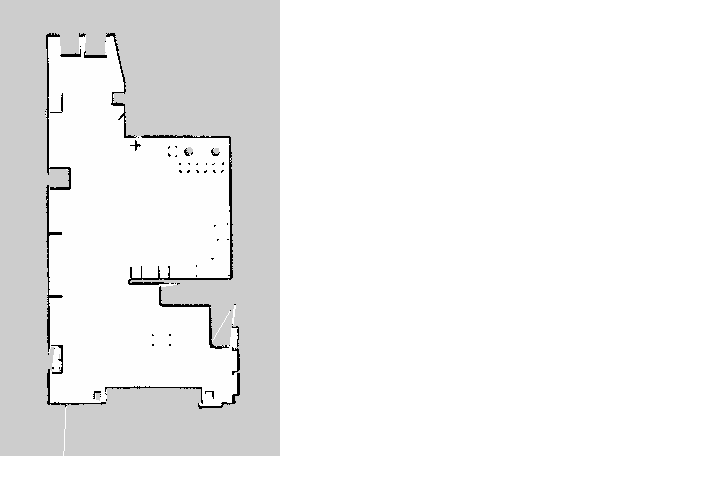
\includegraphics[width=\textwidth]{./img/map_teleop.png}
	\caption{The map that was made through mapping with teleop keyboard package.}
	\label{fig:1:map}
\end{figure}

The transformations are done automatically, as mentioned. It is done through the parameter \t{base_frame} in \t{gmapping}, which has a default called \t{base_link}.

\subsection*{1.b}

For this assignment, the map from the first part had to be reused in Rviz, together with amcl. The following commands were necessary:

\begin{lstlisting}
	roslaunch navigation exercise1.launch
	roslaunch navigation amcl.launch
\end{lstlisting}

This gave a 2D map in Rviz, with an amcl representation of the robot in gazebo, as well as the 3D model in gazebo. In order to try and break the representations of the robot between Rviz and Gazebo, a lot of noise was introduced. Using this meant the rviz robot was at a different point than the gazebo robot after a while.

\lstinputlisting[
	caption={The launch file to map the room.},
	label={lst:2:teleopAmcl}, 
	language=Python,
	float
]{./src/1/amcl.launch}

\lstinputlisting[
	caption={The launch file to map the room.},
	label={lst:3:initPose}, 
	language=Python,
	float
]{./src/1/initPose.py}

The robot its original position had to be changed with python. This can be seen in the listing \ref{lst:3:initPose}. In order to break the AMCL behavior, we played with the noise. As can be seen in listing \ref{lst:2:teleopAmcl}, we change the parameters for \t{odom_alphaN}, with N going from 1 to 4, to $1.5$ instead of $0.2$. This caused the location of the robot in Rviz to occasionally differ from the representation in Gazebo, which could eventually lead to a permanent difference in location.